% =====================================================================================
%  Team Guide -- AI-Powered Smart Home Automation
%  Single-file, Overleaf-compatible (pdfLaTeX). Compile twice for the table of contents.
%  Contains no secrets: only variable NAMES are mentioned, never values.
% =====================================================================================
% api : <GROQ_API_KEY placeholder - set in .env, never commit>
\documentclass[11pt,a4paper]{article}

\usepackage[T1]{fontenc}
\usepackage[utf8]{inputenc}
\usepackage{lmodern}
\usepackage[a4paper,margin=2.4cm]{geometry}
\usepackage{setspace}
\usepackage{amsmath}
\usepackage{xcolor}
\usepackage{tikz}
\usetikzlibrary{arrows.meta,positioning,shapes.geometric,fit,calc}
\usepackage{booktabs,longtable,tabularx,array}
\usepackage{listings}
\usepackage{float}
\usepackage{caption}
\usepackage{enumitem}
\usepackage{fancyhdr}
\usepackage{url}
\usepackage[hidelinks]{hyperref}

\newcommand{\code}[1]{\texttt{\detokenize{#1}}}
\newcommand{\api}[1]{\path{#1}}
\urlstyle{tt}

\setstretch{1.1}
\setlength{\parindent}{0pt}
\setlength{\parskip}{0.45em}
\renewcommand{\arraystretch}{1.15}
\setlist{itemsep=0.15em,topsep=0.25em}
\emergencystretch=3em
\captionsetup{font=small,labelfont=bf}
\setlength{\headheight}{14pt}
\pagestyle{fancy}
\fancyhf{}
\fancyhead[L]{\small Smart Home --- Team Guide}
\fancyfoot[C]{\thepage}

\lstset{basicstyle=\ttfamily\footnotesize,breaklines=true,frame=single,rulecolor=\color{black!35},
  backgroundcolor=\color{black!3},columns=fullflexible,keepspaces=true,showstringspaces=false,language={}}

\tikzset{
  >={Stealth[length=2.2mm]},
  box/.style={draw=black!70, rounded corners=2pt, align=center, font=\footnotesize, inner sep=4pt, minimum height=7mm, fill=blue!6},
  dev/.style={box, fill=orange!14},
  broker/.style={box, fill=green!12},
  store/.style={box, fill=yellow!16},
  ext/.style={box, fill=gray!14, dashed},
  ui/.style={box, fill=purple!9},
  lbl/.style={font=\scriptsize, midway, fill=white, inner sep=1pt},
  flow/.style={->, thick}
}

\title{\textbf{AI-Powered Smart Home Automation}\\[0.3em]\large Team Guide: how the project works and how to work on it}
\author{Prepared for the project team}
\date{Based on the repository state after Chunk 9}

\begin{document}
\maketitle
\tableofcontents
\bigskip

% ------------------------------------------------------------------------------------- 1
\section{Read This First}
\textbf{What it is.} A self-hosted smart-home system. An ESP32-S3 board measures temperature, humidity, motion and raw gas level and sends them over MQTT to a Spring Boot backend that stores them in PostgreSQL. A React website shows everything and lets you control two LEDs, create automation rules, see machine-learning insights, chat with an assistant, and switch Away/Night security modes.

\textbf{The five rules of this codebase.} Keep these in mind before changing anything:
\begin{enumerate}
  \item \textbf{Ownership comes from the login token, never from the request.} Every query is filtered by the owner; somebody else's thing is reported as ``not found'' (HTTP 404).
  \item \textbf{A missing reading is never zero.} Sensor columns are nullable; the UI shows ``no reading''.
  \item \textbf{One path for device commands.} Everything that talks to a device (a person, an automation rule, a security mode) goes through \code{CommandService}.
  \item \textbf{The gas warning LED can never be switched off remotely,} and the real gas warning lives in the firmware, not in the backend. Nothing you add may weaken this.
  \item \textbf{AI and recommendations are advisory.} They may only \emph{propose}; a human must approve before a rule is created.
\end{enumerate}

\begin{center}
\fbox{\parbox{0.94\textwidth}{\small\textbf{Honesty box --- what has and has not been tested.}\\
\textbf{Verified:} 372 automated backend tests pass (in-memory database, fake broker, fake language model); the backend was also run against the real PostgreSQL and Mosquitto containers using \emph{scripts that pretend to be devices}; the frontend builds and lints.\\
\textbf{NOT done:} no physical ESP32-S3 has run the firmware yet; no real large language model (hosted or local) has been used with the assistant (only a scripted fake and a local stub server); the web pages were built and linted but not clicked through by a person in this project; no load or TLS testing. All machine-learning accuracy numbers come from \emph{simulated} data.}}
\end{center}

% ------------------------------------------------------------------------------------- 2
\section{Big Picture}
\begin{figure}[H]
\centering
\resizebox{\textwidth}{!}{%
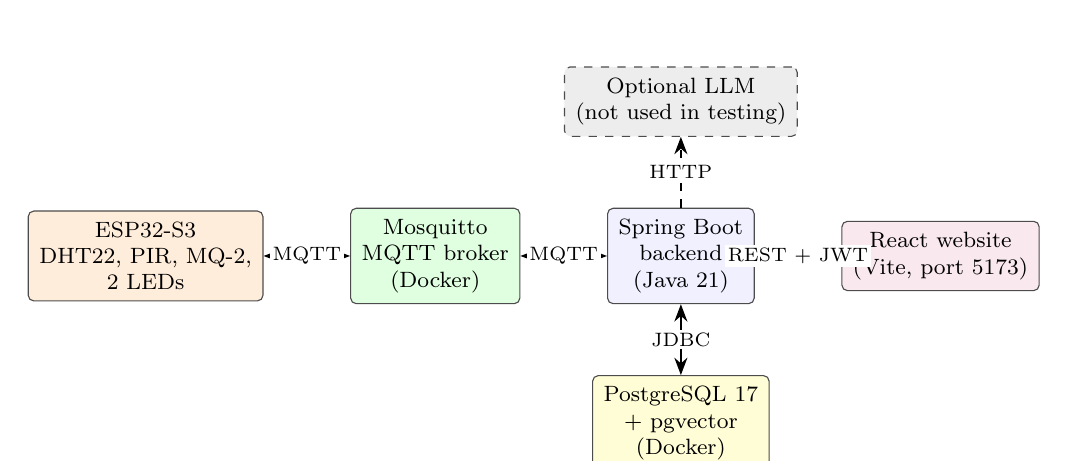
\begin{tikzpicture}[node distance=9mm and 11mm]
  \node[dev] (esp) {ESP32-S3\\DHT22, PIR, MQ-2,\\2 LEDs};
  \node[broker, right=of esp] (mq) {Mosquitto\\MQTT broker\\(Docker)};
  \node[box, right=of mq] (be) {Spring Boot\\backend\\(Java 21)};
  \node[store, below=of be] (db) {PostgreSQL 17\\+ pgvector\\(Docker)};
  \node[ui, right=of be] (web) {React website\\(Vite, port 5173)};
  \node[ext, above=of be] (llm) {Optional LLM\\(not used in testing)};
  \draw[<->, thick] (esp) -- node[lbl]{MQTT} (mq);
  \draw[<->, thick] (mq) -- node[lbl]{MQTT} (be);
  \draw[<->, thick] (be) -- node[lbl]{JDBC} (db);
  \draw[<->, thick] (be) -- node[lbl]{REST + JWT} (web);
  \draw[->, thick, dashed] (be) -- node[lbl]{HTTP} (llm);
\end{tikzpicture}}
\caption{The five parts. Only the LLM is optional and external.}
\end{figure}

The backend is a \emph{modular monolith}: one Java application with one package per feature (no microservices). Packages call each other through their \code{*Service} classes, so ownership checks are written once and reused.

% ------------------------------------------------------------------------------------- 3
\section{Folder Structure}
\begin{lstlisting}
SmartHomeAI/
  backend/                  Spring Boot 4.1.1, Java 21, Maven wrapper (mvnw)
    src/main/java/com/smarthome/<package>/      see section 4
    src/main/resources/
      application.properties                    settings (secrets come from .env)
      db/migration/V1..V9 *.sql                 schema (Flyway) -- the ONLY way to change tables
      db/vendor/postgresql|h2/V8__...sql        vector column (pgvector vs test database)
      assistant/knowledge/*.md                  help text the assistant can search
    src/test/java/com/smarthome/                tests and test fakes
  frontend/                 React 19 + Vite + TypeScript + Tailwind
    src/api.ts              ALL calls to the backend + their TypeScript types
    src/pages/              Login, Register, Dashboard, Devices, Automation,
                            Insights, Assistant
    src/components/         panels (SecurityPanel, TwinPanel, ...), usePolled.ts
  firmware/
    smarthome_esp32s3/      Arduino sketch: config.h, Logic.h, Sensors.*,
                            NetLink.*, CommandParser.h, secrets.example.h
    tests/                  logic_test.cpp, command_test.cpp (run on a PC)
  infra/
    mosquitto/mosquitto.conf       broker config (no anonymous access)
    postgres/init/01-pgvector.sql  enables the vector extension (first start)
  docker-compose.yml        PostgreSQL (pgvector image) + Mosquitto
  .env.example              template for settings -- copy to .env (never commit .env)
  README.md                 detailed per-feature documentation
  main.tex                  the formal project report (LaTeX)
\end{lstlisting}

% ------------------------------------------------------------------------------------- 4
\section{Backend Modules (\code{backend/src/main/java/com/smarthome})}
\begin{longtable}{@{}p{2.6cm}p{4.2cm}p{8.4cm}@{}}
\toprule
\textbf{Package} & \textbf{Key files} & \textbf{What it does}\\
\midrule
\endhead
\code{auth}, \code{user} & \code{AuthController}, \code{AuthService}, \code{JwtService} & Register, login, issue JWT; BCrypt password hashes.\\
\code{device} & \code{DeviceService}, \code{PairingService}, \code{DeviceController}, \code{DevicePairingController}, \code{PairAttemptLimiter} & Devices, one-time pairing codes, ownership, online/offline state, rename, disown (deletes the device's data everywhere).\\
\code{telemetry} & \code{TelemetryIngestService}, \code{TelemetryReading}, \code{TelemetryStoredEvent} & Validates and stores MQTT readings, drops duplicates, announces a stored reading to other modules.\\
\code{mqtt} & \code{MqttIngestClient}, \code{DynsecBrokerAccess}, \code{CommandPublisher} & Paho client (receives telemetry, publishes commands); creates/removes per-device broker accounts.\\
\code{command} & \code{CommandService}, \code{CommandIngestService}, \code{CommandActions}, \code{CommandMaintenance} & LED commands: allow-list, send, acknowledgements, reported LED state, expiry sweeper.\\
\code{automation} & \code{AutomationEngine}, \code{AutomationValidator}, \code{ConditionEvaluator}, \code{AutomationScheduler} & Rules (sensor or schedule triggered), priorities, cooldowns, audit history.\\
\code{ml} & \code{OccupancyTrainer}, \code{LogisticRegression}, \code{AnomalyDetectors}, \code{AnomalyScanner}, \code{MlController} & Occupancy prediction and anomaly detection in plain Java.\\
\code{assistant} & \code{AssistantService}, \code{RagIndexer}, \code{RagChunkStore}, \code{LiveFacts}, \code{PromptBuilder}, \code{GroundingCheck}, \code{HttpLlmClient}, \code{LocalHashEmbedding} & Chat with retrieval (RAG) over the user's own data; rule suggestions that need approval.\\
\code{security} & \code{SecurityService}, \code{SecurityTelemetryListener}, \code{SecurityController} & Home/Away/Night modes, motion alerts, event history.\\
\code{twin} & \code{TwinService}, \code{TwinController} & Compares ``what we asked'' with ``what the device reports''.\\
\code{recommendation} & \code{RecommendationService}, \code{RecommendationController} & Evidence-based suggestions (approve or dismiss).\\
\code{health} & \code{SystemStatusService}, \code{HealthController} & Public \api{/api/health}; logged-in \api{/api/system/status}.\\
\code{config} & \code{SecurityConfig}, \code{GlobalExceptionHandler}, \code{AppConfig} & Two security filter chains (user JWT, device credential), CORS, error-to-HTTP mapping.\\
\bottomrule
\end{longtable}

\textbf{Pattern in every package:} \code{*Controller} (HTTP) $\to$ \code{*Service} (rules, ownership) $\to$ \code{*Repository} (database). DTO records live in \code{*Dtos.java}; custom errors in \code{*Exceptions.java} and are turned into HTTP codes in \code{config/GlobalExceptionHandler.java}.

% ------------------------------------------------------------------------------------- 5
\section{How the Parts Talk to Each Other}
\subsection{Browser to backend}
The website calls \code{fetch} through the helper in \code{frontend/src/api.ts}, which adds \code{Authorization: Bearer <token>}. In development Vite proxies \api{/api} to the backend. A 401 logs the user out. Errors come back as JSON \texttt{\{status, error, message, fieldErrors\}}.

\subsection{Device to backend (MQTT)}
\begin{table}[H]
\centering
\caption{MQTT topics (all under \code{home/devices/<deviceId>/})}
\begin{tabularx}{\textwidth}{llX}
\toprule
\textbf{Suffix} & \textbf{Direction} & \textbf{Meaning}\\
\midrule
\code{telemetry} & device $\to$ backend & Readings, about every 30 s. Not retained.\\
\code{status} & device $\to$ backend & online (retained); Last Will sends offline.\\
\code{commands} & backend $\to$ device & One LED command; QoS 1, never retained. Only the backend may publish here.\\
\code{acks} & device $\to$ backend & \code{applied}, \code{rejected} or \code{expired}.\\
\code{state} & device $\to$ backend & What the LEDs are really doing, plus the gas warning flag.\\
\bottomrule
\end{tabularx}
\end{table}
Each device has its own broker account (username = device id, password = a credential shown once at pairing) that can only touch its own topics. The device identity always comes from the topic, never from the JSON.

Example telemetry (every field except \code{seq} is optional):
\begin{lstlisting}
{ "seq": 42, "temperature": 24.5, "humidity": 55.2, "motion": true, "gasRaw": 1834 }
\end{lstlisting}
\code{gasRaw} is the raw ADC count (0--4095), \textbf{never ppm}.

\subsection{What happens to one reading}
\begin{figure}[H]
\centering
\resizebox{\textwidth}{!}{%
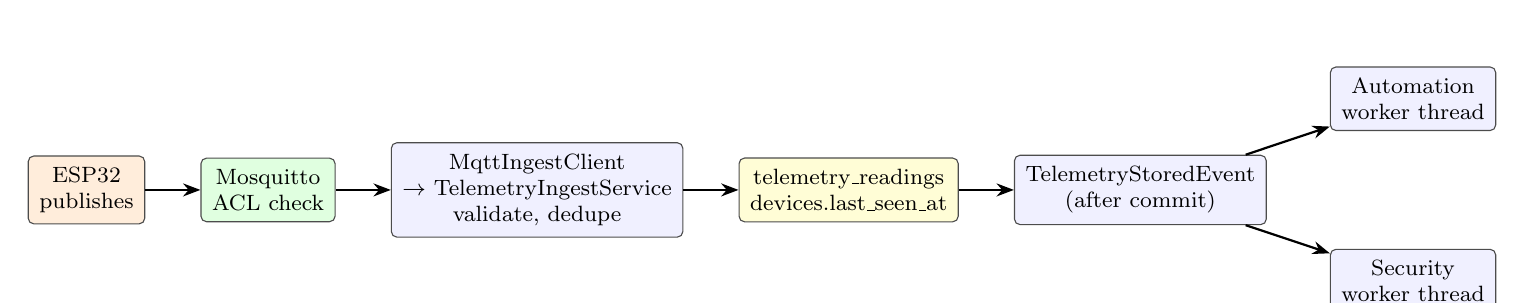
\begin{tikzpicture}[node distance=6mm and 7mm]
  \node[dev] (d) {ESP32\\publishes};
  \node[broker, right=of d] (b) {Mosquitto\\ACL check};
  \node[box, right=of b] (i) {MqttIngestClient\\$\to$ TelemetryIngestService\\validate, dedupe};
  \node[store, right=of i] (db) {telemetry\_readings\\devices.last\_seen\_at};
  \node[box, right=of db] (ev) {TelemetryStoredEvent\\(after commit)};
  \node[box, above right=3mm and 8mm of ev] (a) {Automation\\worker thread};
  \node[box, below right=3mm and 8mm of ev] (s) {Security\\worker thread};
  \draw[flow] (d) -- (b); \draw[flow] (b) -- (i); \draw[flow] (i) -- (db); \draw[flow] (db) -- (ev);
  \draw[flow] (ev) -- (a); \draw[flow] (ev) -- (s);
\end{tikzpicture}}
\caption{Telemetry path. The website later reads the stored rows through the REST API.}
\end{figure}
\textbf{Why worker threads?} Code that runs inside an \code{AFTER_COMMIT} callback and writes to the database silently loses the write. So \code{AutomationDispatcher} and \code{SecurityDispatcher} each run one dedicated thread. Keep this pattern for any new reaction to telemetry.

\subsection{What happens to one command}
\begin{enumerate}
  \item Website: \code{POST /api/devices/<id>/commands} with \texttt{\{action, value\}}.
  \item \code{CommandService} checks: you own the device, it is ONLINE, the action/value is on the allow-list (\code{CommandActions.java}).
  \item The command is saved as PENDING, published to \code{.../commands} (becomes SENT) with an expiry (30 s).
  \item The firmware validates it, changes the LED, replies on \code{.../acks} and reports on \code{.../state} (becomes ACKNOWLEDGED).
  \item No reply by expiry + 10 s $\to$ UNKNOWN (a late ack still fixes it). The website polls the status.
\end{enumerate}
Allowed commands: \code{set_pir_led} = auto/on/off; \code{set_gas_led} = auto/on (\textbf{never off}).

\subsection{Other flows in one line each}
\begin{itemize}
  \item \textbf{Pairing:} user creates a code (valid 10 min, stored hashed) $\to$ types it into the board's Serial Monitor $\to$ board calls \api{/api/device/pair} $\to$ receives its credential once, stores it in flash.
  \item \textbf{Automation:} stored reading $\to$ \code{AutomationEngine} evaluates rules (true/false/\emph{unknown}) $\to$ \code{CommandService} $\to$ audit row in \code{automation_executions}.
  \item \textbf{ML:} training only on request or an hourly check (never per reading); anomaly scan about once a minute.
  \item \textbf{Assistant:} question $\to$ refresh the user's facts from the DB $\to$ embed $\to$ pgvector search (own data only) $\to$ prompt $\to$ LLM $\to$ number/citation check $\to$ answer + sources.
\end{itemize}

% ------------------------------------------------------------------------------------- 6
\section{Database}
Tables are created \emph{only} by Flyway files in \code{db/migration}. Hibernate just validates; if you change an entity you must add a new \code{V10__...sql} (never edit an old one).

\begin{table}[H]
\centering
\caption{Migrations and tables}
\begin{tabularx}{\textwidth}{lX}
\toprule
\textbf{File} & \textbf{Tables}\\
\midrule
V1 & \code{users}\\
V2 & \code{devices}, \code{pairing_codes}\\
V3 & \code{telemetry_readings} (+ presence columns on \code{devices})\\
V4 & \code{device_commands}, \code{device_reported_state}\\
V5 & \code{automation_rules}, \code{automation_conditions}, \code{automation_executions}\\
V6 & \code{ml_models}, \code{ml_anomalies}\\
V7 & \code{rag_chunks}, \code{chat_conversations}, \code{chat_messages}, \code{assistant_suggestions}\\
V8 & \code{embedding} column: pgvector \code{vector} on PostgreSQL (\code{db/vendor/postgresql}), text on H2 for tests\\
V9 & \code{security_settings}, \code{security_events}, \code{recommendations}\\
\bottomrule
\end{tabularx}
\end{table}

\begin{figure}[H]
\centering
\resizebox{0.9\textwidth}{!}{%
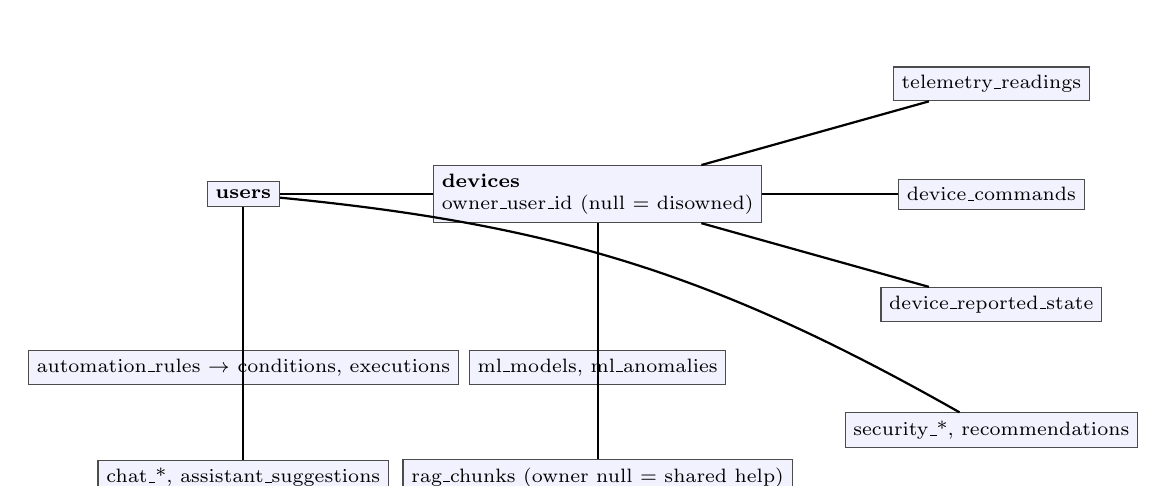
\begin{tikzpicture}
  \tikzset{ent/.style={draw=black!70, align=left, font=\scriptsize, inner sep=3pt, fill=blue!5}}
  \node[ent] (u) at (0,0) {\textbf{users}};
  \node[ent] (d) at (4.5,0) {\textbf{devices}\\owner\_user\_id (null = disowned)};
  \node[ent] (t) at (9.5,1.4) {telemetry\_readings};
  \node[ent] (c) at (9.5,0) {device\_commands};
  \node[ent] (r) at (9.5,-1.4) {device\_reported\_state};
  \node[ent] (a) at (0,-2.2) {automation\_rules $\to$ conditions, executions};
  \node[ent] (m) at (4.5,-2.2) {ml\_models, ml\_anomalies};
  \node[ent] (g) at (0,-3.6) {chat\_*, assistant\_suggestions};
  \node[ent] (k) at (4.5,-3.6) {rag\_chunks (owner null = shared help)};
  \node[ent] (s) at (9.5,-3.0) {security\_*, recommendations};
  \draw[thick] (u) -- (d); \draw[thick] (d) -- (t); \draw[thick] (d) -- (c); \draw[thick] (d) -- (r);
  \draw[thick] (u) -- (a); \draw[thick] (d) -- (m); \draw[thick] (u) -- (g); \draw[thick] (d) -- (k);
  \draw[thick] (u) to[bend left=12] (s);
\end{tikzpicture}}
\caption{Simplified relationships: everything hangs off a user and/or a device. Full diagrams are in the project report (\code{main.tex}).}
\end{figure}
Disowning a device (\code{DeviceService.disown}) deletes its readings, commands, state, rules, models, anomalies, assistant chunks and security events. If you add a table that stores per-device data, \textbf{add its cleanup there}.

% ------------------------------------------------------------------------------------- 7
\section{Important APIs}
All need a user JWT unless marked. The user comes from the token.
\begin{longtable}{@{}p{1.7cm}p{6.6cm}p{6.7cm}@{}}
\toprule
\textbf{Method} & \textbf{Path} & \textbf{Purpose}\\
\midrule
\endhead
GET & \api{/api/health} (public) & Is the backend up?\\
POST & \api{/api/auth/register}, \api{/api/auth/login} (public) & Get a JWT.\\
POST & \api{/api/devices/pairing-codes} & One-time pairing code.\\
POST & \api{/api/device/pair} (device, public) & Board claims itself with the code.\\
GET & \api{/api/devices}, \api{/api/devices/{id}/telemetry} & Devices and readings.\\
DELETE & \api{/api/devices/{id}} & Disown.\\
POST & \api{/api/devices/{id}/commands} & LED command (202; 409 offline; 429 too many).\\
POST, GET & \api{/api/automations} & Create / list rules.\\
GET & \api{/api/automations/executions} & What the rules did and why.\\
POST & \api{/api/devices/{id}/ml/occupancy/train} & Train the occupancy model.\\
GET & \api{/api/devices/{id}/ml/anomalies} & Anomaly list.\\
POST & \api{/api/assistant/chat} & Ask the assistant.\\
POST & \api{/api/assistant/suggestions/{id}/approve} & Turn a suggestion into a rule.\\
PUT & \api{/api/security/mode} & HOME / AWAY / NIGHT.\\
GET & \api{/api/twins} & Digital twins.\\
GET & \api{/api/recommendations} & Suggestions with evidence.\\
GET & \api{/api/system/status} & One-page health of everything.\\
\bottomrule
\end{longtable}
The full list is in the README ("API summary") and in the project report.

% ------------------------------------------------------------------------------------- 8
\section{Setup and Run}
\textbf{You need:} JDK 21+, Node.js 20+, Docker Desktop (running). Maven is bundled (\code{mvnw}).

\begin{lstlisting}
# 1. settings (once). Edit .env: set POSTGRES_PASSWORD, JWT_SECRET (32+ chars),
#    MQTT_ADMIN_PASSWORD, MQTT_BACKEND_PASSWORD. NEVER commit .env or share it.
copy .env.example .env

# 2. database + broker
docker compose up -d
docker compose ps -a          # postgres and mosquitto "Up"; mosquitto-init "Exited (0)" is normal

# 3. backend  (look for "MQTT ingest connected" in the log)
cd backend
.\mvnw.cmd spring-boot:run

# 4. frontend (new terminal)
cd frontend
npm install
npm run dev                   # open the URL Vite prints, register, go to Devices
\end{lstlisting}
Ports already taken on your PC? Change \code{POSTGRES_PORT}, \code{MQTT_PORT} or \code{SERVER_PORT} in \code{.env}. If you change \code{SERVER_PORT}, start the frontend with \code{VITE_API_TARGET} set to the new address and add the frontend origin to \code{CORS_ALLOWED_ORIGINS}.

\textbf{Optional language model for the assistant.} With no \code{LLM_*} variable the assistant still works as a search over your data and says no model is configured. To get written answers set \code{LLM_PROVIDER} (\code{openai} for any OpenAI-compatible server such as Ollama, or \code{anthropic}), \code{LLM_MODEL}, and if needed \code{LLM_BASE_URL}, \code{LLM_API_KEY}, then restart the backend. For meaning-based search also set \code{EMBEDDING_PROVIDER=openai} and \code{EMBEDDING_MODEL}. \textbf{This has not been tried with a real model yet.}

\textbf{Firmware (needs a real board; untested on hardware).} Copy \code{secrets.example.h} to \code{secrets.h} (git-ignored) and fill in Wi-Fi and your PC's LAN address, then:
\begin{lstlisting}
arduino-cli compile --fqbn esp32:esp32:esp32s3 firmware\smarthome_esp32s3
arduino-cli upload  --fqbn esp32:esp32:esp32s3 -p COM5 firmware\smarthome_esp32s3
arduino-cli monitor -p COM5 -c baudrate=115200
\end{lstlisting}
Pins (in \code{config.h}): DHT22 = GPIO14, PIR = GPIO5, PIR LED = GPIO12, MQ-2 analog = GPIO4, gas LED = GPIO13. The MQ-2 AO pin can reach 5~V: power it from 3.3~V or use a voltage divider. The gas thresholds (\code{GAS_WARN_RAW}, \code{GAS_CLEAR_RAW}) are \textbf{placeholders} that must be calibrated.

% ------------------------------------------------------------------------------------- 9
\section{Testing}
\begin{lstlisting}
cd backend;  .\mvnw.cmd verify         # all backend tests (no Docker, no API key needed)
cd frontend; npm run build; npm run lint
cd firmware\tests                      # PC-only firmware logic tests (needs g++), see README
\end{lstlisting}

\subsection{Verified results}
\begin{table}[H]
\centering
\caption{Last full backend run: \code{mvnw verify} = \textbf{372 tests, 0 failures}}
\begin{tabularx}{\textwidth}{lXr}
\toprule
\textbf{Chunk} & \textbf{Main test classes} & \textbf{Tests}\\
\midrule
1--6 & AuthTests, DeviceTests, TelemetryTests, DynsecErrorToleranceTest, CommandTests, ConditionEvaluatorTest, AutomationApiTests, AutomationEngineTests, AutomationScheduleTests, SmarthomeBackendApplicationTests & 137\\
7 (ML) & LogisticRegressionTest, ModelMetricsTest, OccupancyTrainerTest, AnomalyDetectorsTest, MlApiTests, MlAnomalyTests & 79\\
8 (assistant) & ChunkerTest, LocalHashEmbeddingTest, GroundingCheckTest, PromptBuilderTest, SuggestionParserTest, RerankTest, ChatRateLimiterTest, HttpModelClientsTest, AssistantRagTests, AssistantChatTests & 98\\
9 (security etc.) & SecurityModeTests, DigitalTwinTests, RecommendationTests, SystemStatusTests & 58\\
\midrule
 & \textbf{Total} & \textbf{372}\\
\bottomrule
\end{tabularx}
\end{table}
Frontend: \code{npm run build} passes; \code{npm run lint} shows one old cosmetic warning in \code{auth.tsx}.

\subsection{Real versus simulated --- be precise when you talk about results}
\begin{table}[H]
\centering
\caption{What each kind of test really proves}
\begin{tabularx}{\textwidth}{lXX}
\toprule
\textbf{Kind} & \textbf{What it used} & \textbf{What it does \emph{not} prove}\\
\midrule
Unit/integration tests (372) & In-memory H2 database, \code{RecordingCommandPublisher} (fake broker), \code{ScriptedLlm} (fake model), \code{ToggleEmbedding}, \code{SyntheticOccupancy} data & Behaviour with real PostgreSQL features, a real broker, a real model or a real board\\
Live checks on real services & Docker PostgreSQL 17 + pgvector, Docker Mosquitto; Python scripts that \emph{act as devices} using each device's own credential over real MQTT; a local stub server pretending to be an LLM & Anything about physical sensors, Wi-Fi, LEDs, or real LLM answer quality\\
ML numbers & \emph{Simulated} motion/sensor history inserted for the test (e.g. hold-out accuracy 1.000 vs baseline 0.743; 0.99 vs 0.645) & Accuracy in a real home. Perfect scores just mean the made-up pattern is easy.\\
\bottomrule
\end{tabularx}
\end{table}

\subsection{Test helpers you will meet}
\code{AutomationTestBase}, \code{MlTestBase}, \code{AssistantTestBase}, \code{IntelTestBase} (shared setup: register user, pair device, send telemetry through the real ingest code); \code{ScriptedLlm} (script what the ``model'' says and record what it was sent); \code{ToggleRagChunkStore} and \code{ToggleEmbedding} (switch a part ``down'' to test failures). New features should reuse these and test: no login (401), another user's data (404), bad input (400), and the failure path.

% ------------------------------------------------------------------------------------- 10
\section{Debugging Cheat-Sheet}
\begin{longtable}{@{}p{5.2cm}p{9.8cm}@{}}
\toprule
\textbf{Symptom} & \textbf{Try this}\\
\midrule
\endhead
Backend log \code{MQTT not ready ... retrying} & Broker not running or \code{MQTT_*_PASSWORD} does not match the broker volume. \code{docker compose ps -a}; \code{docker logs smarthome-mosquitto}.\\
Device shows \emph{Never connected} & No valid message arrived. Look for \code{Rejected MQTT message} lines in the backend log (they give the reason).\\
Pairing returns 503 & Broker unreachable; nothing changed. Retry with the same code.\\
\code{password authentication failed} though Docker is up & Another PostgreSQL uses the same port. Change \code{POSTGRES_PORT}.\\
Tests/build crash with \code{malloc/mmap failed} & Out of RAM or disk. Close heavy apps and free disk space; crash logs go to \code{backend/target/}.\\
\code{mvnw} fails extracting Maven & Install Maven 3.9+ and use \code{mvn}.\\
Changed DB or broker password after first start & \code{docker compose down -v} resets volumes (\textbf{deletes all data}; devices must be paired again).\\
A new Java file will not compile and looks fine & Check it was not saved with a byte-order mark (BOM) by a tool; save as plain UTF-8.\\
A regex in a Java test behaves strangely & Backslashes in Java strings: use \code{"\\p{Cntrl}"}, not a single backslash escape; a stray \code{\b} became a backspace once.\\
Work done in an \code{AFTER_COMMIT} listener is lost & Hand it to a dispatcher thread (see section 5).\\
Intermittent failures in a test that compares timestamps & Truncate timestamps to microseconds; ties on equal times need an id tie-break (already done in \code{TelemetryRepository}).\\
\bottomrule
\end{longtable}
Useful places to look: backend console (levels INFO/WARN; payloads and secrets are never logged), the \code{automation_executions} table (why a rule did or did not act), \api{/api/system/status} (broker, devices, sensors, commands), and the Serial Monitor on the board (\code{status}, \code{reset}, \code{help}).

% ------------------------------------------------------------------------------------- 11
\section{Current Progress}
\begin{table}[H]
\centering
\caption{Status per chunk}
\begin{tabularx}{\textwidth}{lXl}
\toprule
\textbf{Chunk} & \textbf{Feature} & \textbf{Status}\\
\midrule
1 & Skeleton, Docker, health check & Done, tested\\
2 & Register/login, JWT & Done, tested\\
3 & Pairing, ownership, disown & Done, tested\\
4 & MQTT telemetry, presence & Done, tested (scripted devices)\\
5 & Secure LED commands & Done, tested (scripted devices)\\
6 & Automation engine & Done, tested (scripted devices)\\
7 & ML: occupancy + anomalies & Done, tested on \emph{simulated} data\\
8 & Assistant with RAG & Done; tested with fake/stub model only\\
9 & Security modes, twin, recommendations, status & Done, tested (scripted devices)\\
Firmware & ESP32-S3 sketch & Compiles; PC unit tests; \textbf{never run on a board}\\
\bottomrule
\end{tabularx}
\end{table}

% ------------------------------------------------------------------------------------- 12
\section{Known Limitations}
\begin{itemize}
  \item \textbf{No hardware run.} Sensor accuracy, Wi-Fi behaviour and LED behaviour on a real board are unverified. The firmware LED/gas behaviour was written from scratch (the original sketch was unavailable).
  \item \textbf{Gas thresholds are placeholders;} the gas value is a raw ADC count, not ppm. The system is \textbf{not a certified gas or alarm device}.
  \item \textbf{No real LLM tested.} Answer quality and instruction-following with a real model are unknown. The default embedder matches wording, not meaning.
  \item \textbf{No encryption on the LAN:} MQTT and HTTP are plain; the device credential in flash is not encrypted; the browser keeps the JWT in \code{localStorage}.
  \item \textbf{Hardware ID is not a secret:} a disowned device's id could be re-registered by someone holding a valid pairing code.
  \item \textbf{ML:} ``occupied'' means the PIR fired; one time zone fixed at training; needs about two weeks of real history to be meaningful.
  \item \textbf{Automation:} one flat AND/OR list per rule; a rule watches one device; only the two LEDs can be controlled.
  \item \textbf{Security modes:} no auto schedule, siren or phone notification (alerts are page entries); the ``went offline'' memory is in RAM.
  \item \textbf{UI:} built and linted, not browser-tested; no load testing.
\end{itemize}

% ------------------------------------------------------------------------------------- 13
\section{Remaining Tasks (suggested order)}
\begin{enumerate}
  \item \textbf{Hardware verification} --- follow the 14-step checklist in the README ("Hardware verification checklist"); then calibrate \code{GAS_WARN_RAW}/\code{GAS_CLEAR_RAW} in clean air and with a gas source (safely, ventilated).
  \item \textbf{Try the assistant with a real model} (for example a small local Ollama model, or a hosted API with your own key kept only in \code{.env}); write down retrieval quality and wrong-answer examples.
  \item \textbf{Click through every page} in a browser with a real paired board; fix UI issues; consider adding browser tests.
  \item \textbf{Collect real data for a few weeks,} then retrain the occupancy model and look at the real hold-out metrics.
  \item \textbf{Security hardening:} TLS for MQTT and the API, ESP32 flash encryption, per-device secret at manufacture.
  \item \textbf{Housekeeping:} the README intro still says chatbot/RAG/ML are ``not implemented yet'' --- update that line; keep README and report test counts in sync after every change.
  \item \textbf{Nice to have:} notifications for security alerts, scheduled Night mode, per-device security selection, relay/plug actuators.
\end{enumerate}

% ------------------------------------------------------------------------------------- 14
\section{How to Add a Feature (checklist)}
\begin{enumerate}
  \item New data? Add \code{V10__name.sql} in \code{db/migration}; add the entity and repository; add cleanup to \code{DeviceService.disown} if it is per-device.
  \item Write the \code{*Service} first. Take the owner id as a parameter and filter by it; throw an exception that \code{GlobalExceptionHandler} maps (404 for ``not yours'').
  \item Validate every input; never trust the request for the owner.
  \item If it talks to a device, go through \code{CommandService}; never build a gas-LED ``off''.
  \item Reacting to new telemetry? Use a \code{@TransactionalEventListener} that hands work to a dispatcher thread.
  \item Add the controller, then the type and call in \code{frontend/src/api.ts}, then the panel; give it loading, empty and error states.
  \item Tests: 401, other user's data (404), bad input (400), failure path, then the happy path. Run \code{mvnw verify} and \code{npm run build; npm run lint}.
  \item Update the README section and say honestly what was and was not tested.
\end{enumerate}

\bigskip
\textbf{Secrets reminder.} Never paste passwords, the JWT secret or API keys into code, chats or screenshots. Only \code{.env} (git-ignored) and \code{secrets.h} (git-ignored) hold them.

\end{document}
